% From https://github.com/UWIT-IAM/UWThesis
\documentclass[print]{nuthesis}
\usepackage{amssymb, amsthm, amsmath, amsfonts}
\usepackage{wasysym}
\usepackage{mathrsfs}
% \usepackage{hyperref}
\usepackage{graphicx}
\usepackage{lineno}
\usepackage[colorinlistoftodos]{todonotes}
\usepackage{listings}
%\usepackage{breqn}
\usepackage{cancel, enumerate}
\usepackage{rotating, environ}
\usepackage{caption}
\usepackage{subcaption}
\usepackage[inline]{enumitem}
\usepackage{dirtree}

\newtheorem{thm}{Theorem}
\newtheorem{defn}{Definition}
\newtheorem{prop}{Proposition}
\newtheorem{lemma}{Lemma}
\newtheorem{cor}{Corollary}

% Syntax highlighting #22
  \usepackage{color}
  \usepackage{fancyvrb}
  \newcommand{\VerbBar}{|}
  \newcommand{\VERB}{\Verb[commandchars=\\\{\}]}
  \DefineVerbatimEnvironment{Highlighting}{Verbatim}{commandchars=\\\{\}}
  % Add ',fontsize=\small' for more characters per line
  \usepackage{framed}
  \definecolor{shadecolor}{RGB}{248,248,248}
  \newenvironment{Shaded}{\begin{snugshade}}{\end{snugshade}}
  \newcommand{\AlertTok}[1]{\textcolor[rgb]{0.94,0.16,0.16}{#1}}
  \newcommand{\AnnotationTok}[1]{\textcolor[rgb]{0.56,0.35,0.01}{\textbf{\textit{#1}}}}
  \newcommand{\AttributeTok}[1]{\textcolor[rgb]{0.77,0.63,0.00}{#1}}
  \newcommand{\BaseNTok}[1]{\textcolor[rgb]{0.00,0.00,0.81}{#1}}
  \newcommand{\BuiltInTok}[1]{#1}
  \newcommand{\CharTok}[1]{\textcolor[rgb]{0.31,0.60,0.02}{#1}}
  \newcommand{\CommentTok}[1]{\textcolor[rgb]{0.56,0.35,0.01}{\textit{#1}}}
  \newcommand{\CommentVarTok}[1]{\textcolor[rgb]{0.56,0.35,0.01}{\textbf{\textit{#1}}}}
  \newcommand{\ConstantTok}[1]{\textcolor[rgb]{0.00,0.00,0.00}{#1}}
  \newcommand{\ControlFlowTok}[1]{\textcolor[rgb]{0.13,0.29,0.53}{\textbf{#1}}}
  \newcommand{\DataTypeTok}[1]{\textcolor[rgb]{0.13,0.29,0.53}{#1}}
  \newcommand{\DecValTok}[1]{\textcolor[rgb]{0.00,0.00,0.81}{#1}}
  \newcommand{\DocumentationTok}[1]{\textcolor[rgb]{0.56,0.35,0.01}{\textbf{\textit{#1}}}}
  \newcommand{\ErrorTok}[1]{\textcolor[rgb]{0.64,0.00,0.00}{\textbf{#1}}}
  \newcommand{\ExtensionTok}[1]{#1}
  \newcommand{\FloatTok}[1]{\textcolor[rgb]{0.00,0.00,0.81}{#1}}
  \newcommand{\FunctionTok}[1]{\textcolor[rgb]{0.00,0.00,0.00}{#1}}
  \newcommand{\ImportTok}[1]{#1}
  \newcommand{\InformationTok}[1]{\textcolor[rgb]{0.56,0.35,0.01}{\textbf{\textit{#1}}}}
  \newcommand{\KeywordTok}[1]{\textcolor[rgb]{0.13,0.29,0.53}{\textbf{#1}}}
  \newcommand{\NormalTok}[1]{#1}
  \newcommand{\OperatorTok}[1]{\textcolor[rgb]{0.81,0.36,0.00}{\textbf{#1}}}
  \newcommand{\OtherTok}[1]{\textcolor[rgb]{0.56,0.35,0.01}{#1}}
  \newcommand{\PreprocessorTok}[1]{\textcolor[rgb]{0.56,0.35,0.01}{\textit{#1}}}
  \newcommand{\RegionMarkerTok}[1]{#1}
  \newcommand{\SpecialCharTok}[1]{\textcolor[rgb]{0.00,0.00,0.00}{#1}}
  \newcommand{\SpecialStringTok}[1]{\textcolor[rgb]{0.31,0.60,0.02}{#1}}
  \newcommand{\StringTok}[1]{\textcolor[rgb]{0.31,0.60,0.02}{#1}}
  \newcommand{\VariableTok}[1]{\textcolor[rgb]{0.00,0.00,0.00}{#1}}
  \newcommand{\VerbatimStringTok}[1]{\textcolor[rgb]{0.31,0.60,0.02}{#1}}
  \newcommand{\WarningTok}[1]{\textcolor[rgb]{0.56,0.35,0.01}{\textbf{\textit{#1}}}}

%% https://github.com/rstudio/rmarkdown/issues/1649
\newlength{\cslhangindent}
\setlength{\cslhangindent}{1.5em}
\newenvironment{CSLReferences}[2]%
{\setlength{\parindent}{0pt}%
\everypar{\setlength{\hangindent}{\cslhangindent}}\ignorespaces}%
{\par}

% fix for pandoc 1.14
\providecommand{\tightlist}{%
  \setlength{\itemsep}{0pt}\setlength{\parskip}{0pt}}

%% something about tables, from https://github.com/ismayc/thesisdown/issues/122
\usepackage{calc}

%% for copyright symbol
\usepackage{textcomp}

%% to allow to rotate pages to landscape
\usepackage{lscape}
%% to adjust table column width
\usepackage{tabularx}

% suppress bottom page numbers on first page of each chapter
% because they overlap with text
\usepackage{etoolbox}
\patchcmd{\chapter}{plain}{empty}{}{}

%% for more attractive tables
\usepackage{booktabs}
\usepackage{longtable}


\usepackage{graphicx}


% Double spacing, if you want it.
\def\dsp{\def\baselinestretch{2.0}\large\normalsize}
% \dsp

% If the Grad. Division insists that the first paragraph of a section
% be indented (like the others), then include this line:
\usepackage{indentfirst}

%%%%%%%%%%%%%%%%%%
% If you want to use "sections" to partition your thesis
% un-comment the following:
%
% \counterwithout{section}{chapter}
% \setsecnumdepth{subsubsection}
% \def\sectionmark#1{\markboth{#1}{#1}}
% \def\subsectionmark#1{\markboth{#1}{#1}}
% \renewcommand{\thesection}{\arabic{section}}
% \renewcommand{\thesubsection}{\thesection.\arabic{subsection}}
% \makeatletter
% \let\l@subsection\l@section
% \let\l@section\l@chapter
% \makeatother

\renewcommand{\thetable}{\arabic{table}}
\renewcommand{\thefigure}{\arabic{figure}}

%%%%%%%%%%%%%%%%%%


%% Stuff from https://github.com/suchow/Dissertate

% The following line would print the thesis in a postscript font

% \usepackage{natbib}
% \def\bibpreamble{\protect\addcontentsline{toc}{chapter}{Bibliography}}

\setcounter{tocdepth}{1} % Print the chapter and sections to the toc
% controls depth of table of contents (toc): 0 = chapter, 1 = section, 2 = subsection

\usepackage{natbib}


% commands and environments needed by pandoc snippets
% extracted from the output of `pandoc -s`
%% Make R markdown code chunks work
\usepackage{array}
\usepackage{amssymb,amsmath}
\usepackage{ifxetex,ifluatex}
\ifxetex
  \usepackage{fontspec,xltxtra,xunicode}
  \defaultfontfeatures{Mapping=tex-text,Scale=MatchLowercase}
\else
  \ifluatex
    \usepackage{fontspec}
    \defaultfontfeatures{Mapping=tex-text,Scale=MatchLowercase}
  \else
    \usepackage[utf8]{inputenc}
  \fi
\fi
\usepackage{color}
\usepackage{fancyvrb}


\ifxetex
  \usepackage[setpagesize=false, % page size defined by xetex
              unicode=false, % unicode breaks when used with xetex
              xetex,
              colorlinks=true,
              linkcolor=blue]{hyperref}
\else
  \usepackage[unicode=true,
              colorlinks=true,
              linkcolor=blue]{hyperref}
\fi
\hypersetup{breaklinks=true, pdfborder={0 0 0}}
\setlength{\parindent}{20pt}
\setlength{\parskip}{6pt plus 2pt minus 1pt}
\setlength{\emergencystretch}{3em}  % prevent overfull lines
\setcounter{secnumdepth}{2} %% controls section numbering, e.g. 1 or 1.2, or 1.2.3


\input{preamble.tex}

\begin{document}
% \linenumbers{}
%% Start formatting the first few special pages
%% frontmatter is needed to set the page numbering correctly
\frontmatter
%% from thesisdown
% To pass between YAML and LaTeX the dollar signs are added by CII
\title{STATISTICAL TESTING OF ACTIVITY CLIFFS}
\author{Sarah Josephine Aurit}
\adviser{Souparno Ghosh}
% \adviserAbstract{}
\major{Statistics}
\degreemonth{December}
\degreeyear{2023}
% \copyrightpage
%%
%% For most people the defaults will be correct, so they are commented
%% out. To manually set these, just uncomment and make the needed
%% changes.
%% \college{Your college}
%% \city{Your City}
%%
%% For most people the following can be changed with a class
%% option. To manually set these, just uncomment the following and
%% make the needed changes.
%% \doctype{Thesis or Dissertation}
%% \degree{Your degree}
%% \degreeabbreviation{Your degree abbr.}
%%
%% Now that we know everything we need, we can generate the title page
%% itself.
%%
\maketitle


\begin{abstract}
    Here is my abstract. \emph{(350 word limit)}
\end{abstract}

%% Optional
\begin{copyrightpage}
\end{copyrightpage}

%% Optional
\begin{dedication}
Dedicated to\ldots{}
\end{dedication}

%%%%%%%%%%%%%%%%%%%
% Acknowledgments
%%%%%%%%%%%%%%%%%%%
\begin{acknowledgments}
I am grateful for this second opportunity from the University of Nebraska-Lincoln to pursue further education. I am more appreciative of the academic journey, which includes meeting so many new and inspiring individuals including my fellow students, professors, and advisor and exposure to new and cutting edge content to sharpen my statistical skillset. The journey mirrored other aspects of life in which I had to discover that with enough hard work that many things are possible, and that I still have a contribution to make within multiple realms of life.

Thank you Dr.~Stroup for giving me the confidence to continue moving forward in the work. Dr.~Eskridge you were an inspiration and I learned so much from you. Dr.~Ghosh, thank you for taking me on when you already had so many students.

To my most beloved children, you are cherished beyond words and I hope this endeavour proves fruitful for us as a family in the years to come. You were patient with me, and I hope that I have shown you a small portion of what is possible in your own life.
\end{acknowledgments}
%%%%%%%%%%%%%%%%%%%

%%%%%%%%%%%%%%%%%%%
% Grant Information
%%%%%%%%%%%%%%%%%%%
% \begin{grantinfo}
%     % Add any grant info here
% \end{grantinfo}

%%%%%%%%%%%%%%%%%%%
% ToC
%%%%%%%%%%%%%%%%%%%
\tableofcontents

%%%%%%%%%%%%%%%%%%%
% List of Figures
%%%%%%%%%%%%%%%%%%%
\listoffigures
\listoftables

%%%%%%%%%%%%%%%%%%%
% Start of the document
%%%%%%%%%%%%%%%%%%%
\mainmatter


\hypertarget{literature-review}{%
\chapter{Literature Review}\label{literature-review}}

\hypertarget{motivation-and-background}{%
\section{Motivation and Background}\label{motivation-and-background}}

The journey of discovering effective cancer drugs can be long and expensive. The elements of time and cost weigh against the race to improve survival and the quality of life for cancer patients. Researchers typically start testing drug compounds on cancer cell lines within a laboratory setting first before testing on animals or humans. To narrow the search field, drugs are sometimes pursued that are similar to ones previously found to be successful in cancer treatment. That said, it is possible for the similar drug to be much less effective, which is defined as an activity cliff (AC) (Cruz-Monteagudo et al., 2014).

According to HU et al.~(2017), compounds that are structurally similar yet have large potency differences are identified as producing activity cliffs upon an activity landscape. Additionally, an activity cliff is potentially produced within the context of the following four key aspects: 1) we are considering and comparing a pair of compounds, 2) both compounds are active against the same target, 3) the two compounds are similar in chemical structure, and 4) there is a difference in potency.

Focusing on the aspect of compound similarity via cheminformatics, formal investigation is completed by looking at similarity measurements. There are multiple approaches regarding the quantification of similarity between two compounds. One popular selection is the Tanimoto coefficient.

The Tanimoto coefficient, a measure of similarity, is determined by the quantification of molecular attributes that are similar between two molecular compounds. Essentially, it is a ratio of the number of similar entities divided by the total number of molecular attributes. (Reference: Why is Tanimoto index an appropriate choice for fingerprint-based similarity calculations?)

Analogously, matched molecular pairs (MMP) analysis encompasses another measurement of similarity. Essentially, two molecules differ by one ``well-defined, structural'' chemical transformation. (Reference: \url{https://pubs-acs-org.libproxy.unl.edu/doi/pdf/10.1021/jm200452d}). MMPs were initially used as a special case of a quantitative structure-activity relationship (QSAR), which relates molecular compounds to the response of potency or other biochemical properties.

QSAR methodology can be essential in determining the relationships between chemical structures and biochemical activities, and it is typical that the methodology incorporates supervised machine learning techniques. Compounds are first represented by a numerical entity such as a two-dimensional structural formula that promulgates atom connectivity via chemical bonds. The structural formula then is related to bioactivities. It is not uncommon for there to be violations of QSAR methodology given the presence of an AC. (Reference: QSAR modeling where have you been where are you going)

\hypertarget{gdsc-dataset}{%
\section{GDSC Dataset}\label{gdsc-dataset}}

The Genomics of Drug Sensitivity in Cancer (GDSC) database was instituted by the UK's Wellcome Sanger Institute's Cancer Genome Project and Massachusetts General Hospital's Center for Molecular Therapeutics. It is a repository and compilation of anti-cancer drug response information for more than 100 drugs linked to almost 700 cancer cell lines of multiple primary cancer sites for a total of approximately 75,000 experiments. Fluorescence-based assays were obtained after 72 hours had elapsed to measure drug sensitivity for each experiment. The response was quantified by \(IC_\text{50}\), a metric that reveals how much substance or dose is necessary to inhibit a biological component by 50\%. Additionally, the slope of the dose-response curve fitted to nine drug concentrations and area under the curve (AUC) were reported as additional measures of sensitivity (Reference: Genomics of Drug Sensitivity in Cancer: A Resource for Therapeutic Biomarker Discovery in Cancer Cells).

We focus on breast cancer data, which is populated by data linked to over 200 drugs. Disregarding missing data, approximately 900 drug characteristics were identified for each drug alongside the mean values of the log of \(IC_\text{50}\) values.

\hypertarget{transformation}{%
\section{Transformation}\label{transformation}}

Dimension reduction is a critical element in the investigation of these breast cancer drugs because of the high dimensionality of drug characteristics relative to the number of drugs. Classical techniques such as principal component analysis (PCA) and multidimensional scaling (MDS) rely on the assumptions that fail within the context of non-linear structures that are intrinsic to some datasets. An alternative dimension reduction technique is that of isometric feature mapping (isomap). \url{https://wearables.cc.gatech.edu/paper_of_week/isomap.pdf} The algorithm is comprised of three steps. First, Euclidean distances are calculated at each point for all other points that are either within a specific radius or are considered a \(K\) nearest neighbors (\(k\)NN), which are utilized to construct a distance matrix. Next, all pairwise distances are calculated and the shortest path is selected by Dijkstra's (shortest pathway from one node to another while navigating intermediary nodes) or Floyd-Warshall algorithm.

Large Margin Nearest Neighbor (LMNN) was a subsequent methodology to promote improvement of grouping like drug responses. LMNN allows for learning more appropriate distances via transformation of the two dimensional coordinates obtained from the isomap dimension reduction technique.

\hypertarget{stationarity-for-irregularly-spaced-data}{%
\section{Stationarity for Irregularly Spaced Data}\label{stationarity-for-irregularly-spaced-data}}

We can consider the investigation of drug efficacy over molecular space within the context of spatial statistics. Commonly, assumptions surrounding spatial data include that of second-order stationarity to make accurate predictions. We consider drug efficacy as a random variable for each known position within molecular space. The first requirement for second-order stationarity is that the expectation and variance of drug efficacy is constant over the entire domain of molecular space. An additional requirement is that the covariance between any two observations only relies on the distance between the two observations. We denote a spatial process in \(d\) dimensions, and where \(\textbf{s}\) is the location in two dimensions post-dimension reduction. Also, let \(Z(\textbf{s})\) be the realization of a process, and let \(Z(\textbf{s})\) be a random variable, which is indexed by its location \(\textbf{s} \in R^\text{2}\). We can then define constant expectation and covariance over the domain of molecular space:

\begin{equation}
  E[Z(\textbf{s})]=\mu 
\end{equation} \begin{equation}
  cov[{Z(\textbf{s}_\text1),Z(\textbf{s}_\text2)}]=c(\textbf{s}_\text1, \textbf{s}_\text2) 
\end{equation}

Bandyopadhyya and Rao (2017), proposed a test for second order stationarity for irregularly spaced data for the region \([-\lambda/2, \lambda/2]^\text{2}\) assuming the locations are independent and uniformly distributed random variables. An adaptation of the classical discrete Fourier transforms (DFTs) of a time series for a spatial random field is as follows for \((\textbf{s}_j,Z(\textbf{s}_j); j = 1,...,n)\) observations:

\begin{equation}
  J_n(\boldsymbol{\omega})=\frac{\lambda^{d/2}}{n}\sum_{j=1}^{n}Z(\textbf{s}_j)exp(i\textbf{s}_j'\boldsymbol{\omega}) 
\end{equation}

Given the fact that we have locations of points within a grid of two dimensions, the equation simplifies to:

\begin{equation}
  J_n(\omega_k)=\frac{\lambda}{n}\sum_{j=1}^{n}Z(s_{j_1}, s_{j_2})\omega_k 
\end{equation}

With \(2\pi\) periodicity (in each dimension?), the fundamental frequency is \(2\pi/\lambda\). The aggregation of terms incorporates frequencies \(\omega_k = exp[\frac{2\pi i}{\lambda}(s_{j_1}k_1+s_{j_2}k_2)]\) to transform the sequence of \(Z(s_j)\) observations to the DFTs where i is \(\sqrt{-1}\). In matrix form:

\begin{equation}
  J_n(\omega) = \frac{\lambda}{n}
 \begin{bmatrix}
    1 & 1 & 1 & \cdots & 1 \\
    1 & \omega_k & \omega_k^2 & \cdots & \omega_k^{(n-1)} \\
    1 & \omega_k^2 & \omega_k^4 & \cdots & \omega_k^{2(n-1)} \\
    \vdots \\
    1 & \omega_k^{(n-1)} & \omega_k^{2(n-1)} & \cdots & \omega_k^{(n-1)(n-1)} 
  \end{bmatrix}
  \begin{bmatrix}
      \hat{Z(s_{1_1}, s_{1_2})} \\
      \hat{Z(s_{2_1}, s_{2_2})} \\
      \hat{Z(s_{3_1}, s_{3_2})} \\
      \vdots \\
      \hat{Z(s_{n_1}, s_{n_2})}
  \end{bmatrix}
\end{equation}

In order to examine stationarity vs.~non-stationarity, we construct a test statistic to investigate the null hypothesis that the spatial field is second-order stationary as opposed to non-stationary (observed - expected?). The first component of the statistic is the measurement of covariance between the DFTs and a lag \(r\):

\begin{equation}
\begin{split}
  \hat{A}_\lambda(g;r)&=\frac{1}{\lambda^{d}}\sum_{k_1,\cdots,k_d=-a}^{a}g(\omega_k)J_n(\omega_k)\overline{J_n(\omega_{k+r})}\\
  &-\frac{1}{n}\sum_{k_1,...,k_d=-a}^{a}g(\omega_k) x \frac{1}{n}\sum_{j=1}^{n}Z(s_j)^2exp(-is'_j\omega_r)
\end{split}
\end{equation}

where \(g\) is a Lipschitz continuous function. The test statistic is then constructed from this as follows to reflect:

\begin{equation}
  T_S=\frac{\lambda^d max_{\left(r \epsilon S\right)}{\left\lvert\hat{A}_\lambda\left(g;r\right) \right\rvert}^2} {c_{\left(\lambda,1\right)}}
\end{equation}

where \(S\) is a finite set that surrounds the origin, and \(S \cap S' =\emptyset\).

The estimation of \(c_{\lambda,1}\) that estimates variance is as follows:

\begin{equation}
  \hat{c}_{\lambda}(S')=\frac{\lambda^d}{2|S'|-1}\sum_{r \epsilon S'}[({\mathscr{R} \hat{A}_\lambda(g;r)-\overline{A}})^2+({\mathscr{I} \hat{A}_\lambda(g;r)-\overline{A}})^2]
\end{equation}

where \(S' \epsilon Z^d/ \{0\}\) and \(\overline{A}={{1/2|S'|}}\sum_{r \epsilon S'}({\mathscr{R} \hat{A}_\lambda(g;r)+\mathscr{I} \hat{A}_\lambda(g;r)})\). It is intuitive to think that When lag \(r\) that is close to zero, the coefficients \(\hat{A}\) have similar variance.

We investigate second-order stationarity for the GDSC data consisting of 208 drugs applied to breast cancer cell lines and the response of log\(IC_\text{50}\). We initially employ three scenarios that differ based on lambda value (\(\lambda = 1, 2, and 10\) with a consistent grid pattern in that there are the same number of total grid elements with \(k_1 , k_2\) incrementally indexed by a factor of ten. For each scenario, we look at the data before and after transformation in conjunction with each of the three scenarios and present the T test statistic and associated p-values.

\hypertarget{results}{%
\section{Results}\label{results}}

We recognize a distinct pattern change in the comparison of pre- and post-transformation coordinates and associated outcome values for the largest two-dimensional grid space (Figures 1.1 and 1.2). For all positive coordinates and before transformation, we see evidence of \(\mathscr{R} \hat{A}_\lambda\) and \(\mathscr{I} \hat{A}_\lambda\) values associated with statistical significance (the real and imaginary \(\hat{A}_\lambda\) values comprise the numerator of the global test statistic). The count of \(\mathscr{R} \hat{A}_\lambda\) and \(\mathscr{I} \hat{A}_\lambda\) values that fall outside of the interval {[}-1.75, 1.75{]} when considering a \(t\)-distribution with 15? degrees of freedom (could include a graphic that showcases the appropriate degrees of freedom S and S') decrease from three to one from pre- to post-transformation. Additionally, the pre-transformation test statistic and associated \(P\)-value (T=8.49; \(P\)=0.125) also differs from the post-transformation test statistic and \(P\)-value (T=3.85; \(P\)=0.508). We assume a Gaussian process with exponential covariance.

\begin{figure}[tbp]

{\centering 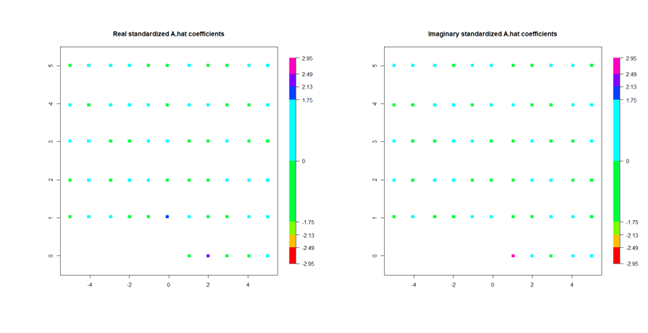
\includegraphics[width=\linewidth,]{figure/Stationarity_Apre_l10_k10} 

}

\caption{Pre-Transformation; $\lambda=10$}\label{fig:unnamed-chunk-1}
\end{figure}

\begin{figure}[tbp]

{\centering 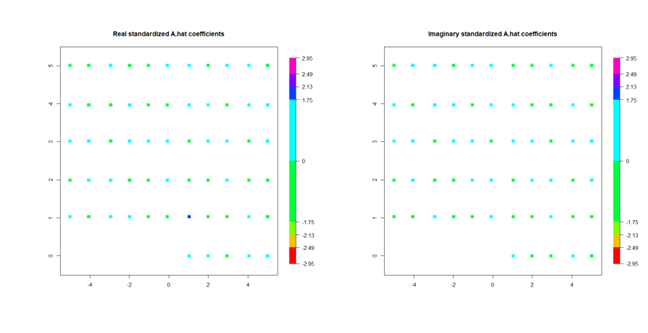
\includegraphics[width=\linewidth,]{figure/Stationarity_Apost_l10_k10} 

}

\caption{Post-Transformation; $\lambda=10$}\label{fig:unnamed-chunk-2}
\end{figure}

As we zoom in, all statistical evidence of non-stationarity is eliminated, and there are no further indication that \(\mathscr{R} \hat{A}_\lambda\) and \(\mathscr{I} \hat{A}_\lambda\) values fall outside the interval {[}-1.75, 1.75{]}.

\begin{figure}[tbp]

{\centering 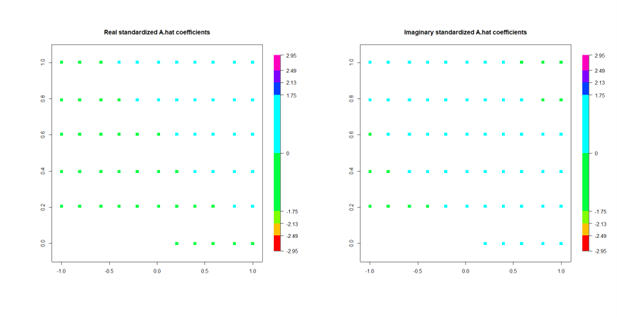
\includegraphics[width=\linewidth,]{figure/Stationarity_Apre_l2_k10} 

}

\caption{Pre-Transformation; $\lambda=2$}\label{fig:unnamed-chunk-3}
\end{figure}

\begin{figure}[tbp]

{\centering 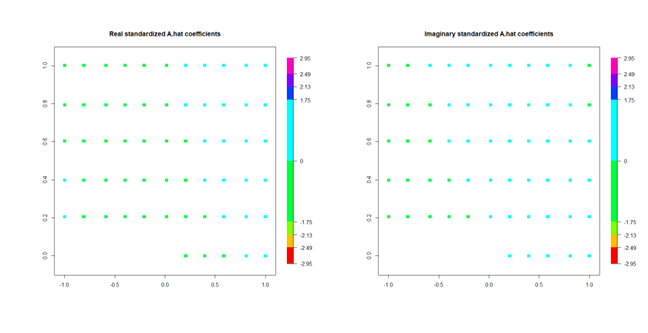
\includegraphics[width=\linewidth,]{figure/Stationarity_Apost_l2_k10} 

}

\caption{Post-Transformation; $\lambda=2$}\label{fig:unnamed-chunk-4}
\end{figure}

\begin{figure}[tbp]

{\centering 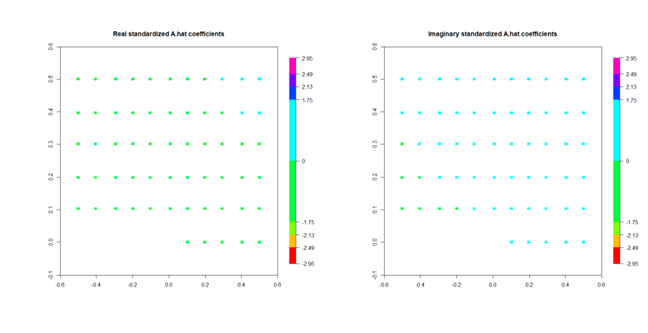
\includegraphics[width=\linewidth,]{figure/Stationarity_Apre_l1_k10} 

}

\caption{Pre-Transformation; $\lambda=1$}\label{fig:unnamed-chunk-5}
\end{figure}

\begin{figure}[tbp]

{\centering 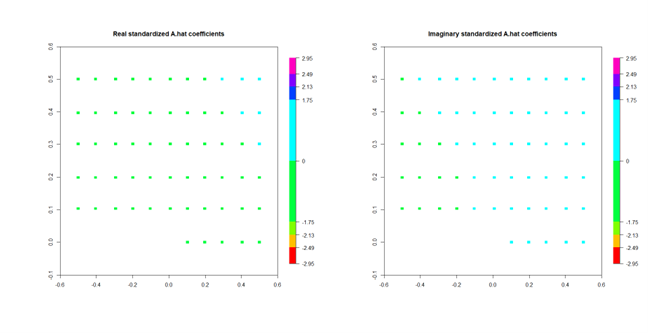
\includegraphics[width=\linewidth,]{figure/Stationarity_Apost_l1_k10} 

}

\caption{Post-Transformation; $\lambda=1$}\label{fig:unnamed-chunk-6}
\end{figure}

With similar degrees of freedom, the pre- and post-transformation test statistic and associated \(P\)-values when \(\lambda=2\) (Pre-Transformation: T=2.06; \(P\)=0.808 and Post-Transformation: T=2.56; \(P\)=0.727) and \(\lambda=1\) (Pre-Transformation: T=2.19; \(P\)=0.795 and Post-Transformation: T=2.36; \(P\)=0.764) are all scenarios that show statistical evidence of second-order stationarity. Upon examination of the plots of the real and imaginary components on the positive points of the grid, we see confirmation that stationarity is present.

\hypertarget{discussion-and-conclusion}{%
\section{Discussion and Conclusion}\label{discussion-and-conclusion}}

The investigation of second order stationarity is relevant when considering the potential of an activity cliff. We hypothesize that an AC will be associated with statistical evidence of a violation of second-order stationarity.

\hypertarget{rmd-basics}{%
\chapter{R Markdown Basics}\label{rmd-basics}}

Here is a brief introduction into using \emph{R Markdown}. \emph{Markdown} is a simple formatting syntax for authoring HTML, PDF, and MS Word documents. \emph{R Markdown} provides the flexibility of \emph{Markdown} with the implementation of \textbf{R} input and output. For more details on using \emph{R Markdown} see \url{http://rmarkdown.rstudio.com}.

Be careful with your spacing in \emph{Markdown} documents. While whitespace largely is ignored, it does at times give \emph{Markdown} signals as to how to proceed. As a habit, try to keep everything left aligned whenever possible, especially as you type a new paragraph. In other words, there is no need to indent basic text in the Rmd document (in fact, it might cause your text to do funny things if you do).

\hypertarget{lists}{%
\section{Lists}\label{lists}}

It's easy to create a list. It can be unordered like

\begin{itemize}
\tightlist
\item
  Item 1
\item
  Item 2
\end{itemize}

or it can be ordered like

\begin{enumerate}
\def\labelenumi{\arabic{enumi}.}
\tightlist
\item
  Item 1
\item
  Item 2
\end{enumerate}

Notice that I intentionally mislabeled Item 2 as number 4. \emph{Markdown} automatically figures this out! You can put any numbers in the list and it will create the list. Check it out below.

To create a sublist, just indent the values a bit (at least four spaces or a tab). (Here's one case where indentation is key!)

\begin{enumerate}
\def\labelenumi{\arabic{enumi}.}
\tightlist
\item
  Item 1
\item
  Item 2
\item
  Item 3

  \begin{itemize}
  \tightlist
  \item
    Item 3a
  \item
    Item 3b
  \end{itemize}
\end{enumerate}

\hypertarget{line-breaks}{%
\section{Line breaks}\label{line-breaks}}

Make sure to add white space between lines if you'd like to start a new paragraph. Look at what happens below in the outputted document if you don't:

Here is the first sentence. Here is another sentence. Here is the last sentence to end the paragraph.
This should be a new paragraph.

\emph{Now for the correct way:}

Here is the first sentence. Here is another sentence. Here is the last sentence to end the paragraph.

This should be a new paragraph.

\hypertarget{r-chunks}{%
\section{R chunks}\label{r-chunks}}

When you click the \textbf{Knit} button above a document will be generated that includes both content as well as the output of any embedded \textbf{R} code chunks within the document. You can embed an \textbf{R} code chunk like this (\texttt{cars} is a built-in \textbf{R} dataset):

\begin{verbatim}
##      speed           dist       
##  Min.   : 4.0   Min.   :  2.00  
##  1st Qu.:12.0   1st Qu.: 26.00  
##  Median :15.0   Median : 36.00  
##  Mean   :15.4   Mean   : 42.98  
##  3rd Qu.:19.0   3rd Qu.: 56.00  
##  Max.   :25.0   Max.   :120.00
\end{verbatim}

\hypertarget{inline-code}{%
\section{Inline code}\label{inline-code}}

If you'd like to put the results of your analysis directly into your discussion, add inline code like this:

\begin{quote}
The \texttt{cos} of \(2 \pi\) is 1.
\end{quote}

Another example would be the direct calculation of the standard deviation:

\begin{quote}
The standard deviation of \texttt{speed} in \texttt{cars} is 5.2876444.
\end{quote}

One last neat feature is the use of the \texttt{ifelse} conditional statement which can be used to output text depending on the result of an \textbf{R} calculation:

\begin{quote}
The standard deviation is less than 6.
\end{quote}

Note the use of \texttt{\textgreater{}} here, which signifies a quotation environment that will be indented.

As you see with \texttt{\$2\ \textbackslash{}pi\$} above, mathematics can be added by surrounding the mathematical text with dollar signs. More examples of this are in \protect\hyperlink{math-sci}{Mathematics and Science} if you uncomment the code in \protect\hyperlink{math}{Math}.

\hypertarget{including-plots}{%
\section{Including plots}\label{including-plots}}

You can also embed plots. For example, here is a way to use the base \textbf{R} graphics package to produce a plot using the built-in \texttt{pressure} dataset:

\begin{center}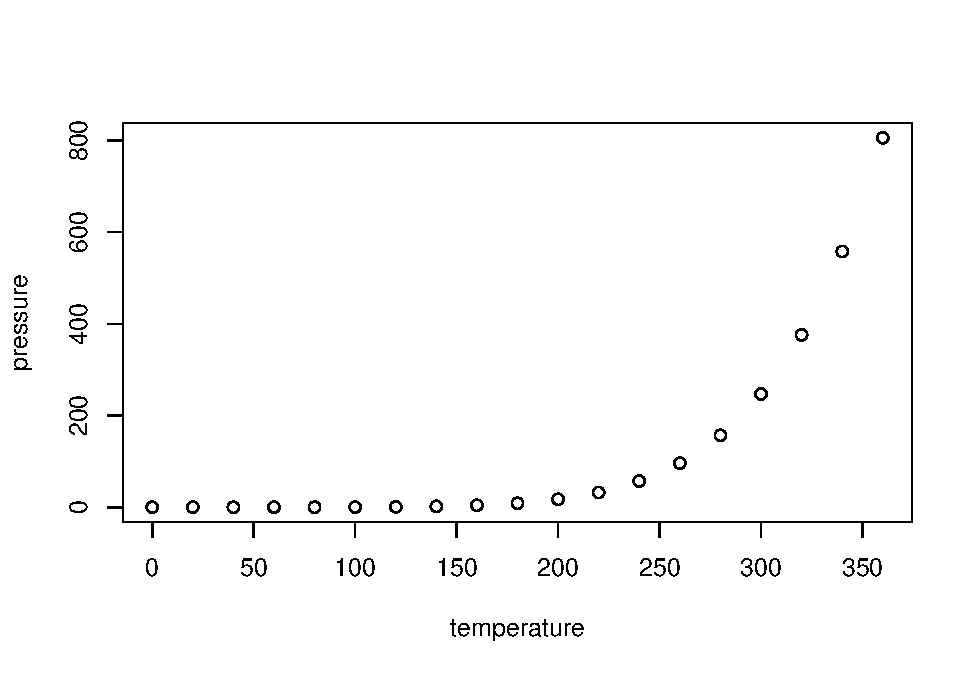
\includegraphics[width=\linewidth,]{thesis_files/figure-latex/pressure-1} \end{center}

Note that the \texttt{echo=FALSE} parameter was added to the code chunk to prevent printing of the \textbf{R} code that generated the plot. There are plenty of other ways to add chunk options. More information is available at \url{http://yihui.name/knitr/options/}.

Another useful chunk option is the setting of \texttt{cache=TRUE} as you see here. If document rendering becomes time consuming due to long computations or plots that are expensive to generate you can use knitr caching to improve performance. Later in this file, you'll see a way to reference plots created in \textbf{R} or external figures.

\hypertarget{loading-and-exploring-data}{%
\section{Loading and exploring data}\label{loading-and-exploring-data}}

Included in this template is a file called \texttt{flights.csv}. This file includes a subset of the larger dataset of information about all flights that departed from Seattle and Portland in 2014. More information about this dataset and its \textbf{R} package is available at \url{http://github.com/ismayc/pnwflights14}. This subset includes only Portland flights and only rows that were complete with no missing values. Merges were also done with the \texttt{airports} and \texttt{airlines} data sets in the \texttt{pnwflights14} package to get more descriptive airport and airline names.

We can load in this data set using the following command:

The data is now stored in the data frame called \texttt{flights} in \textbf{R}. To get a better feel for the variables included in this dataset we can use a variety of functions. Here we can see the dimensions (rows by columns) and also the names of the columns.

\begin{verbatim}
## [1] 52808    16
\end{verbatim}

\begin{verbatim}
##  [1] "month"        "day"          "dep_time"    
##  [4] "dep_delay"    "arr_time"     "arr_delay"   
##  [7] "carrier"      "tailnum"      "flight"      
## [10] "dest"         "air_time"     "distance"    
## [13] "hour"         "minute"       "carrier_name"
## [16] "dest_name"
\end{verbatim}

Another good idea is to take a look at the dataset in table form. With this dataset having more than 50,000 rows, we won't explicitly show the results of the command here. I recommend you enter the command into the Console \textbf{\emph{after}} you have run the \textbf{R} chunks above to load the data into \textbf{R}.

While not required, it is highly recommended you use the \texttt{dplyr} package to manipulate and summarize your data set as needed. It uses a syntax that is easy to understand using chaining operations. Below I've created a few examples of using \texttt{dplyr} to get information about the Portland flights in 2014. You will also see the use of the \texttt{ggplot2} package, which produces beautiful, high-quality academic visuals.

We begin by checking to ensure that needed packages are installed and then we load them into our current working environment:

\clearpage

The example we show here does the following:

\begin{itemize}
\item
  Selects only the \texttt{carrier\_name} and \texttt{arr\_delay} from the \texttt{flights} dataset and then assigns this subset to a new variable called \texttt{flights2}.
\item
  Using \texttt{flights2}, we determine the largest arrival delay for each of the carriers.
\end{itemize}

A useful function in the \texttt{knitr} package for making nice tables in \emph{R Markdown} is called \texttt{kable}. It is much easier to use than manually entering values into a table by copying and pasting values into Excel or LaTeX. This again goes to show how nice reproducible documents can be! (Note the use of \texttt{results="asis"}, which will produce the table instead of the code to create the table.) The \texttt{caption.short} argument is used to include a shorter title to appear in the List of Tables.

\begin{longtable}[t]{lr}
\caption[Max Delays by Airline]{\label{tab:maxdelays}Maximum Delays by Airline}\\
\toprule
Airline & Max Arrival Delay\\
\midrule
Alaska Airlines Inc. & 338\\
American Airlines Inc. & 1539\\
Delta Air Lines Inc. & 651\\
Frontier Airlines Inc. & 575\\
Hawaiian Airlines Inc. & 407\\
\addlinespace
JetBlue Airways & 273\\
SkyWest Airlines Inc. & 421\\
Southwest Airlines Co. & 694\\
United Air Lines Inc. & 472\\
US Airways Inc. & 347\\
\addlinespace
Virgin America & 366\\
\bottomrule
\end{longtable}

The last two options make the table a little easier-to-read.

We can further look into the properties of the largest value here for American Airlines Inc.~To do so, we can isolate the row corresponding to the arrival delay of 1539 minutes for American in our original \texttt{flights} dataset.

\begin{verbatim}
##   dep_time dep_delay arr_time tailnum flight dest air_time
## 1     1403      1553     1934  N595AA   1568  DFW      182
##   distance
## 1     1616
\end{verbatim}

We see that the flight occurred on March 3rd and departed a little after 2 PM on its way to Dallas/Fort Worth. Lastly, we show how we can visualize the arrival delay of all departing flights from Portland on March 3rd against time of departure.

\begin{center}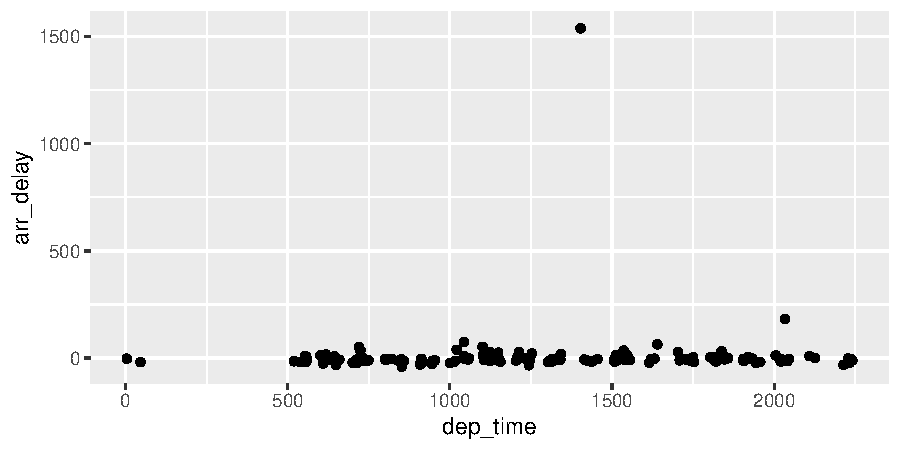
\includegraphics[width=\linewidth,]{thesis_files/figure-latex/march3plot-1} \end{center}

\hypertarget{additional-resources}{%
\section{Additional resources}\label{additional-resources}}

\begin{itemize}
\item
  \emph{Markdown} Cheatsheet - \url{https://github.com/adam-p/markdown-here/wiki/Markdown-Cheatsheet}
\item
  \emph{R Markdown} Reference Guide - \url{https://www.rstudio.com/wp-content/uploads/2015/03/rmarkdown-reference.pdf}
\item
  Introduction to \texttt{dplyr} - \url{https://cran.rstudio.com/web/packages/dplyr/vignettes/introduction.html}
\item
  \texttt{ggplot2} Documentation - \url{http://docs.ggplot2.org/current/}
\end{itemize}

\hypertarget{math-sci}{%
\chapter{Mathematics and Science}\label{math-sci}}

\hypertarget{math}{%
\section{Math}\label{math}}

\TeX~is the best way to typeset mathematics. Donald Knuth designed \TeX~when he got frustrated at how long it was taking the typesetters to finish his book, which contained a lot of mathematics. One nice feature of \emph{R Markdown} is its ability to read LaTeX code directly.

If you are doing a thesis that will involve lots of math, you will want to read the following section which has been commented out. If you're not going to use math, skip over or delete this next commented section.

\noindent Exponent or Superscript: \(\mathrm{O^-}\)

\noindent Subscript: \(\mathrm{CH_4}\)

To stack numbers or letters as in \(\mathrm{Fe_2^{2+}}\), the subscript is defined first, and then the superscript is defined.

\noindent Bullet: CuCl \(\bullet\) \(\mathrm{7H_{2}O}\)

\noindent Delta: \(\Delta\)

\noindent Reaction Arrows: \(\longrightarrow\) or \(\xrightarrow{solution}\)

\noindent Resonance Arrows: \(\leftrightarrow\)

\noindent Reversible Reaction Arrows: \(\rightleftharpoons\)

\hypertarget{typesetting-reactions}{%
\subsection{Typesetting reactions}\label{typesetting-reactions}}

You may wish to put your reaction in an equation environment, which means that LaTeX will place the reaction where it fits and will number the equations for you.

\begin{equation}
  \mathrm{C_6H_{12}O_6  + 6O_2} \longrightarrow \mathrm{6CO_2 + 6H_2O}
  \label{eq:reaction}
\end{equation}

We can reference this combustion of glucose reaction via Equation \eqref{eq:reaction}.

\hypertarget{conclusion}{%
\chapter*{Conclusion}\label{conclusion}}
\addcontentsline{toc}{chapter}{Conclusion}

If we don't want Conclusion to have a chapter number next to it, we can add the \texttt{\{-\}} attribute.

\textbf{More info}

And here's some other random info: the first paragraph after a chapter title or section head \emph{shouldn't be} indented, because indents are to tell the reader that you're starting a new paragraph. Since that's obvious after a chapter or section title, proper typesetting doesn't add an indent there.

\appendix

\hypertarget{the-first-appendix}{%
\chapter{The First Appendix}\label{the-first-appendix}}

This first appendix includes all of the R chunks of code that were hidden throughout the document (using the \texttt{include\ =\ FALSE} chunk tag) to help with readibility and/or setup.

\textbf{In the main Rmd file}

\begin{Shaded}
\begin{Highlighting}[]
\CommentTok{\# This chunk ensures that the huskydown}
\CommentTok{\# package is installed and loaded. This}
\CommentTok{\# huskydown package includes the template}
\CommentTok{\# files for the thesis.}
\ControlFlowTok{if}\NormalTok{ (}\SpecialCharTok{!}\FunctionTok{require}\NormalTok{(devtools)) }\FunctionTok{install.packages}\NormalTok{(}\StringTok{"devtools"}\NormalTok{,}
    \AttributeTok{repos =} \StringTok{"http://cran.rstudio.com"}\NormalTok{)}
\ControlFlowTok{if}\NormalTok{ (}\SpecialCharTok{!}\FunctionTok{require}\NormalTok{(huskydown)) devtools}\SpecialCharTok{::}\FunctionTok{install\_github}\NormalTok{(}\StringTok{"benmarwick/huskydown"}\NormalTok{)}
\FunctionTok{library}\NormalTok{(huskydown)}
\FunctionTok{library}\NormalTok{(tidyverse)}
\FunctionTok{library}\NormalTok{(knitr)}
\FunctionTok{library}\NormalTok{(ggplot2)}
\FunctionTok{library}\NormalTok{(formatR)}
\end{Highlighting}
\end{Shaded}

\textbf{In Chapter \ref{ref-labels}:}

\hypertarget{the-second-appendix-for-fun}{%
\chapter{The Second Appendix, for Fun}\label{the-second-appendix-for-fun}}

\hypertarget{colophon}{%
\chapter*{Colophon}\label{colophon}}
\addcontentsline{toc}{chapter}{Colophon}

This document is set in \href{https://github.com/georgd/EB-Garamond}{EB Garamond}, \href{https://github.com/adobe-fonts/source-code-pro/}{Source Code Pro} and \href{http://www.latofonts.com/lato-free-fonts/}{Lato}. The body text is set at 11pt with \(\familydefault\).

It was written in R Markdown and \(\LaTeX\), and rendered into PDF using \href{https://github.com/benmarwick/huskydown}{huskydown} and \href{https://github.com/rstudio/bookdown}{bookdown}.

This document was typeset using the XeTeX typesetting system, and the \href{http://staff.washington.edu/fox/tex/}{University of Washington Thesis class} class created by Jim Fox. Under the hood, the \href{https://github.com/UWIT-IAM/UWThesis}{University of Washington Thesis LaTeX template} is used to ensure that documents conform precisely to submission standards. Other elements of the document formatting source code have been taken from the \href{https://github.com/stevenpollack/ucbthesis}{Latex, Knitr, and RMarkdown templates for UC Berkeley's graduate thesis}, and \href{https://github.com/suchow/Dissertate}{Dissertate: a LaTeX dissertation template to support the production and typesetting of a PhD dissertation at Harvard, Princeton, and NYU}

The source files for this thesis, along with all the data files, have been organised into an R package, xxx, which is available at \url{https://github.com/xxx/xxx}. A hard copy of the thesis can be found in the University of Washington library.

This version of the thesis was generated on 2023-03-15 00:05:38. The repository is currently at this commit:

The computational environment that was used to generate this version is as follows:

\begin{verbatim}
## - Session info -------------------------------------------
##  setting  value
##  version  R version 4.2.1 (2022-06-23 ucrt)
##  os       Windows 10 x64 (build 22000)
##  system   x86_64, mingw32
##  ui       RTerm
##  language (EN)
##  collate  English_United States.utf8
##  ctype    English_United States.utf8
##  tz       America/Chicago
##  date     2023-03-15
##  pandoc   2.18 @ C:/Program Files/RStudio/bin/quarto/bin/tools/ (via rmarkdown)
## 
## - Packages -----------------------------------------------
##  package       * version date (UTC) lib source
##  assertthat      0.2.1   2019-03-21 [1] CRAN (R 4.2.2)
##  backports       1.4.1   2021-12-13 [1] CRAN (R 4.2.0)
##  bookdown        0.31.2  2023-01-09 [1] Github (rstudio/bookdown@604939c)
##  broom           1.0.2   2022-12-15 [1] CRAN (R 4.2.2)
##  cachem          1.0.6   2021-08-19 [1] CRAN (R 4.2.2)
##  callr           3.7.3   2022-11-02 [1] CRAN (R 4.2.2)
##  cellranger      1.1.0   2016-07-27 [1] CRAN (R 4.2.2)
##  cli             3.4.1   2022-09-23 [1] CRAN (R 4.2.2)
##  colorspace      2.0-3   2022-02-21 [1] CRAN (R 4.2.2)
##  crayon          1.5.2   2022-09-29 [1] CRAN (R 4.2.2)
##  DBI             1.1.3   2022-06-18 [1] CRAN (R 4.2.2)
##  dbplyr          2.2.1   2022-06-27 [1] CRAN (R 4.2.2)
##  devtools      * 2.4.5   2022-10-11 [1] CRAN (R 4.2.2)
##  digest          0.6.31  2022-12-11 [1] CRAN (R 4.2.2)
##  dplyr         * 1.0.10  2022-09-01 [1] CRAN (R 4.2.2)
##  ellipsis        0.3.2   2021-04-29 [1] CRAN (R 4.2.2)
##  evaluate        0.19    2022-12-13 [1] CRAN (R 4.2.2)
##  fansi           1.0.3   2022-03-24 [1] CRAN (R 4.2.2)
##  farver          2.1.1   2022-07-06 [1] CRAN (R 4.2.2)
##  fastmap         1.1.0   2021-01-25 [1] CRAN (R 4.2.2)
##  forcats       * 0.5.2   2022-08-19 [1] CRAN (R 4.2.2)
##  formatR       * 1.14    2023-01-17 [1] CRAN (R 4.2.2)
##  fs              1.5.2   2021-12-08 [1] CRAN (R 4.2.2)
##  gargle          1.2.1   2022-09-08 [1] CRAN (R 4.2.2)
##  generics        0.1.3   2022-07-05 [1] CRAN (R 4.2.2)
##  ggplot2       * 3.4.0   2022-11-04 [1] CRAN (R 4.2.2)
##  git2r           0.30.1  2022-03-16 [1] CRAN (R 4.2.2)
##  glue            1.6.2   2022-02-24 [1] CRAN (R 4.2.2)
##  googledrive     2.0.0   2021-07-08 [1] CRAN (R 4.2.2)
##  googlesheets4   1.0.1   2022-08-13 [1] CRAN (R 4.2.2)
##  gtable          0.3.1   2022-09-01 [1] CRAN (R 4.2.2)
##  haven           2.5.1   2022-08-22 [1] CRAN (R 4.2.2)
##  hms             1.1.2   2022-08-19 [1] CRAN (R 4.2.2)
##  htmltools       0.5.4   2022-12-07 [1] CRAN (R 4.2.2)
##  htmlwidgets     1.6.1   2023-01-07 [1] CRAN (R 4.2.2)
##  httpuv          1.6.7   2022-12-14 [1] CRAN (R 4.2.2)
##  httr            1.4.4   2022-08-17 [1] CRAN (R 4.2.2)
##  huskydown     * 0.0.5   2022-12-20 [1] Github (benmarwick/huskydown@addb48e)
##  jsonlite        1.8.4   2022-12-06 [1] CRAN (R 4.2.2)
##  knitr         * 1.41    2022-11-18 [1] CRAN (R 4.2.2)
##  labeling        0.4.2   2020-10-20 [1] CRAN (R 4.2.0)
##  later           1.3.0   2021-08-18 [1] CRAN (R 4.2.2)
##  lifecycle       1.0.3   2022-10-07 [1] CRAN (R 4.2.2)
##  lubridate       1.9.0   2022-11-06 [1] CRAN (R 4.2.2)
##  magrittr        2.0.3   2022-03-30 [1] CRAN (R 4.2.2)
##  memoise         2.0.1   2021-11-26 [1] CRAN (R 4.2.2)
##  mime            0.12    2021-09-28 [1] CRAN (R 4.2.0)
##  miniUI          0.1.1.1 2018-05-18 [1] CRAN (R 4.2.2)
##  modelr          0.1.10  2022-11-11 [1] CRAN (R 4.2.2)
##  munsell         0.5.0   2018-06-12 [1] CRAN (R 4.2.2)
##  pillar          1.8.1   2022-08-19 [1] CRAN (R 4.2.2)
##  pkgbuild        1.4.0   2022-11-27 [1] CRAN (R 4.2.2)
##  pkgconfig       2.0.3   2019-09-22 [1] CRAN (R 4.2.2)
##  pkgload         1.3.2   2022-11-16 [1] CRAN (R 4.2.2)
##  prettyunits     1.1.1   2020-01-24 [1] CRAN (R 4.2.2)
##  processx        3.8.0   2022-10-26 [1] CRAN (R 4.2.2)
##  profvis         0.3.7   2020-11-02 [1] CRAN (R 4.2.2)
##  promises        1.2.0.1 2021-02-11 [1] CRAN (R 4.2.2)
##  ps              1.7.2   2022-10-26 [1] CRAN (R 4.2.2)
##  purrr         * 1.0.0   2022-12-20 [1] CRAN (R 4.2.2)
##  R6              2.5.1   2021-08-19 [1] CRAN (R 4.2.2)
##  Rcpp            1.0.9   2022-07-08 [1] CRAN (R 4.2.2)
##  readr         * 2.1.3   2022-10-01 [1] CRAN (R 4.2.2)
##  readxl          1.4.1   2022-08-17 [1] CRAN (R 4.2.2)
##  remotes         2.4.2   2021-11-30 [1] CRAN (R 4.2.2)
##  reprex          2.0.2   2022-08-17 [1] CRAN (R 4.2.2)
##  rlang           1.0.6   2022-09-24 [1] CRAN (R 4.2.2)
##  rmarkdown       2.19    2022-12-15 [1] CRAN (R 4.2.2)
##  rstudioapi      0.14    2022-08-22 [1] CRAN (R 4.2.2)
##  rvest           1.0.3   2022-08-19 [1] CRAN (R 4.2.2)
##  scales          1.2.1   2022-08-20 [1] CRAN (R 4.2.2)
##  sessioninfo     1.2.2   2021-12-06 [1] CRAN (R 4.2.2)
##  shiny           1.7.4   2022-12-15 [1] CRAN (R 4.2.2)
##  stringi         1.7.8   2022-07-11 [1] CRAN (R 4.2.1)
##  stringr       * 1.5.0   2022-12-02 [1] CRAN (R 4.2.2)
##  tibble        * 3.1.8   2022-07-22 [1] CRAN (R 4.2.2)
##  tidyr         * 1.2.1   2022-09-08 [1] CRAN (R 4.2.2)
##  tidyselect      1.2.0   2022-10-10 [1] CRAN (R 4.2.2)
##  tidyverse     * 1.3.2   2022-07-18 [1] CRAN (R 4.2.2)
##  timechange      0.2.0   2023-01-11 [1] CRAN (R 4.2.2)
##  tzdb            0.3.0   2022-03-28 [1] CRAN (R 4.2.2)
##  urlchecker      1.0.1   2021-11-30 [1] CRAN (R 4.2.2)
##  usethis       * 2.1.6   2022-05-25 [1] CRAN (R 4.2.2)
##  utf8            1.2.2   2021-07-24 [1] CRAN (R 4.2.2)
##  vctrs           0.5.1   2022-11-16 [1] CRAN (R 4.2.2)
##  withr           2.5.0   2022-03-03 [1] CRAN (R 4.2.2)
##  xfun            0.35    2022-11-16 [1] CRAN (R 4.2.2)
##  xml2            1.3.3   2021-11-30 [1] CRAN (R 4.2.2)
##  xtable          1.8-4   2019-04-21 [1] CRAN (R 4.2.2)
##  yaml            2.3.6   2022-10-18 [1] CRAN (R 4.2.2)
## 
##  [1] C:/Program Files/R/R-4.2.1/library
## 
## ----------------------------------------------------------
\end{verbatim}

\backmatter

\hypertarget{references}{%
\chapter*{References}\label{references}}
\addcontentsline{toc}{chapter}{References}

\noindent

\setlength{\parindent}{-0.20in}
\setlength{\leftskip}{0.20in}
\setlength{\parskip}{8pt}

\hypertarget{refs}{}
\begin{CSLReferences}{1}{0}
\leavevmode\vadjust pre{\hypertarget{ref-angel2000}{}}%
Angel, E. (2000). \emph{Interactive computer graphics : A top-down approach with OpenGL}. Boston, MA: Addison Wesley Longman.

\leavevmode\vadjust pre{\hypertarget{ref-angel2001}{}}%
Angel, E. (2001a). \emph{Batch-file computer graphics : A bottom-up approach with QuickTime}. Boston, MA: Wesley Addison Longman.

\leavevmode\vadjust pre{\hypertarget{ref-angel2002a}{}}%
Angel, E. (2001b). \emph{Test second book by angel}. Boston, MA: Wesley Addison Longman.

\end{CSLReferences}


%% backmatter is needed at the end of the main body of your thesis to
%% set up page numbering correctly for the remainder of the thesis
\backmatter

%% Start the correct formatting for the appendices
% \appendix
%% Input each appendix here
% \input{./appendix_a}

%% Bibliography goes here (You better have one)
%% BibTeX is your friend

% \bibliographystyle{alpha}  % or use  abbrv to abbreviate first names and use numerical indices
\bibliographystyle{abbrv}  % or use  abbrv to abbreviate first names and use numerical indices
%% Add your BibTex file here (don't include the .bib)
\bibliography{./references}



%% Index go here (if you have one)
\end{document}
